\documentclass[12pt,letterpaper,titlepage,en-US]{article}

\usepackage{basicstyle}
\usepackage{report}
%\usepackage{knit}

\usepackage{listings}
\usepackage{xcolor}


\definecolor{codegreen}{rgb}{0,0.6,0}
\definecolor{codegray}{rgb}{0.5,0.5,0.5}
\definecolor{codepurple}{rgb}{0.58,0,0.82}
\definecolor{backcolour}{rgb}{0.95,0.95,0.92}
 
\lstdefinestyle{mystyle}{
    backgroundcolor=\color{backcolour},   
    commentstyle=\color{codegreen},
    keywordstyle=\color{magenta},
    numberstyle=\tiny\color{codegray},
    stringstyle=\color{codepurple},
    basicstyle=\ttfamily\footnotesize,
    breakatwhitespace=false,         
    breaklines=true,                 
    captionpos=b,                    
    keepspaces=true,                 
    numbers=left,                    
    numbersep=5pt,                  
    showspaces=false,                
    showstringspaces=false,
    showtabs=false,                  
    tabsize=2
}
 
\lstset{style=mystyle}



\usepackage[toc,page]{appendix}

\newcommand{\hmwkTitle}{Project \#2}
\DTMsavetimestamp{DueDate}{2019-11-05T11:59:00+00:00}
\newcommand{\hmwkClass}{CS 6385.001}
\newcommand{\hmwkClassName}{Algorithmic Aspects of Telecommunication Networks}
\newcommand{\hmwkClassInstructor}{Instructor: Prof. Andras Farago}
\newcommand{\hmwkAuthorName}{Shyam Patharla}
\newcommand{\hmwkAuthorNetID}{sxp178231}




%
% Title Page
%

\title{
    \vspace{1in}
    \textmd{\textbf{\hmwkClassName \\\hmwkClass:\ \hmwkTitle }}\\
    \normalsize\vspace{0.1in}\small{Due\ on\ \DTMusedate{DueDate}\ at \DTMusetime{DueDate} }\\
    \vspace{0.1in}\large{\textit{\hmwkClassInstructor}}\\
    \vspace{0.5in}
\includegraphics[height=2.4em]{UTD_logo_BW}\\
    \vspace{2in}
}

\author{\textbf{\hmwkAuthorName\ \footnotesize{(\hmwkAuthorNetID)}} \\ }
\date{}
\makeindex

\begin{document}
\maketitle
\pagenumbering{Roman}

\tableofcontents

\pagebreak
\pagenumbering{arabic}

\section{Introduction}
\begin{itemize}
\item In this project, we try to implement the Nagamochi Ibaraki algorithm for finding the edge connectivity of a connected graph
\item Give an input graph with n nodes and m edges, our program outputs the edge connectivity of the graph
\item We do this for range of values of m
\item  We also analyze how the edge connectivity varies with the value of m and assess the spread of the edge connectivity values
\item We discuss the possible reasons for the above characteristics.
\end{itemize}

\section{Design Decisions}
\begin{itemize}
\item We implement the solution in the \textbf{Java} programming language
\item The program modules were run on a \textbf{Mac} operating system

\end{itemize}





\section{Solution Approach}

\subsection{Generating Input Examples}
\textit{Module 1} consists of generating input graphs for simulating the algorithm.
These parameters are then passed on to second module which runs the Nagamochi Ibaraki  algorithm on them. The graphs are generated as follows.

\begin{itemize}
\item For all examples, we set the number of nodes in the network to 20 i.e \textit{n} = 20.

\item The number of edges is taken from the set [19,190] in steps of 3 i.e. m=19,22,25,....190

\item For each pair of values of m and n we generate 5 graphs

\item  The m edges are selected randomly 
\item Self loops and parallel edges are avoided.



\end{itemize}




\subsection{Nagamochi Ibaraki Algorithm}
Module 2 receives input parameters from the first module (graph). It has the following functions.

\begin{itemize}

\item \textbf{isConnected()} 
\begin{itemize}
\item checks if the input graph is connected using depth-first search
\item If the input graph is disconnected, its edge connectivity is zero
\end{itemize}


\item \textbf{runAlgorithm()}
\begin{itemize}
\item Runs the Nagamochi Ibaraki algorithm on an input graph
\item If there are only two nodes in the graph, the number of edges between the two nodes is the edge connectivity
\item If the number of nodes in the current graph is greater than 2, we run the \textit{maximum adjacency ordering} algorithm
\item Compute the \textbf{degree} between the last node in the ordering
\item The last two nodes in the ordering are merged
\item The \textbf{edge connectivity} of the \textit{merged graph} is computed recursively
\item The edge connectivity of the graph is minimum of the values of the two values

\end{itemize}





\item \textbf{maximumAdjacency()}
\begin{itemize}
\item Returns the maximum adjacency ordering of the nodes in the current graph.
\item The first node in the ordering is chosen \textit{randomly}
\item Given the first k nodes ($v_{1},v_{2},...v_{k}$) are chosen, the node which has the \textit{maximum} edges to the set ($v_{1},...v_{k}$) is chosen to be $v_{k+1}$
\end{itemize}


\item \textbf{contractGraph()}
\begin{itemize}
\item Contracts two nodes in a graph
\item All resulting self loops are removed 
\item Parallel edges are kept
\end{itemize}


\item \textbf{dfs()}
\begin{itemize}
\item Runs a depth first search on a graph
\end{itemize}



\end{itemize}

Modul2 2 computes the edge connectivity of an input graph and passes it on to Module 3.




\subsection{Presentation of Results}
\begin{itemize}

\item \textit{Module 3} takes the output parameters of \textit{Module 2} i.e. the \textbf{edge connectivity} for a graph with n nodes and m edges

\item For each value of m we had generated 5 graphs. The edge connectivity for that value of m is the \textbf{average} of the edge connectivities of these 5 graphs

 \item The above computation is repeated for all \textbf{m} values in the range [19,190] in steps of 3

\item We compute the \textbf{spread} of the each edge connectivity value. 

\item The \textit{spread} of an edge connectivity value is the difference between the smallest and largest value of m for which the value occurs.
 

 
\item We then try to answer questions such as:
\begin{itemize}
\item How does the \textbf{edge connectivity} of the network vary with the value of \textbf{m}?
\item How does \textbf{spread} of an edge connectivity value vary with the value of the \textbf{edge connectivity}? 
\end{itemize}




\item We present the execution of our project using the flow chart below.\\

  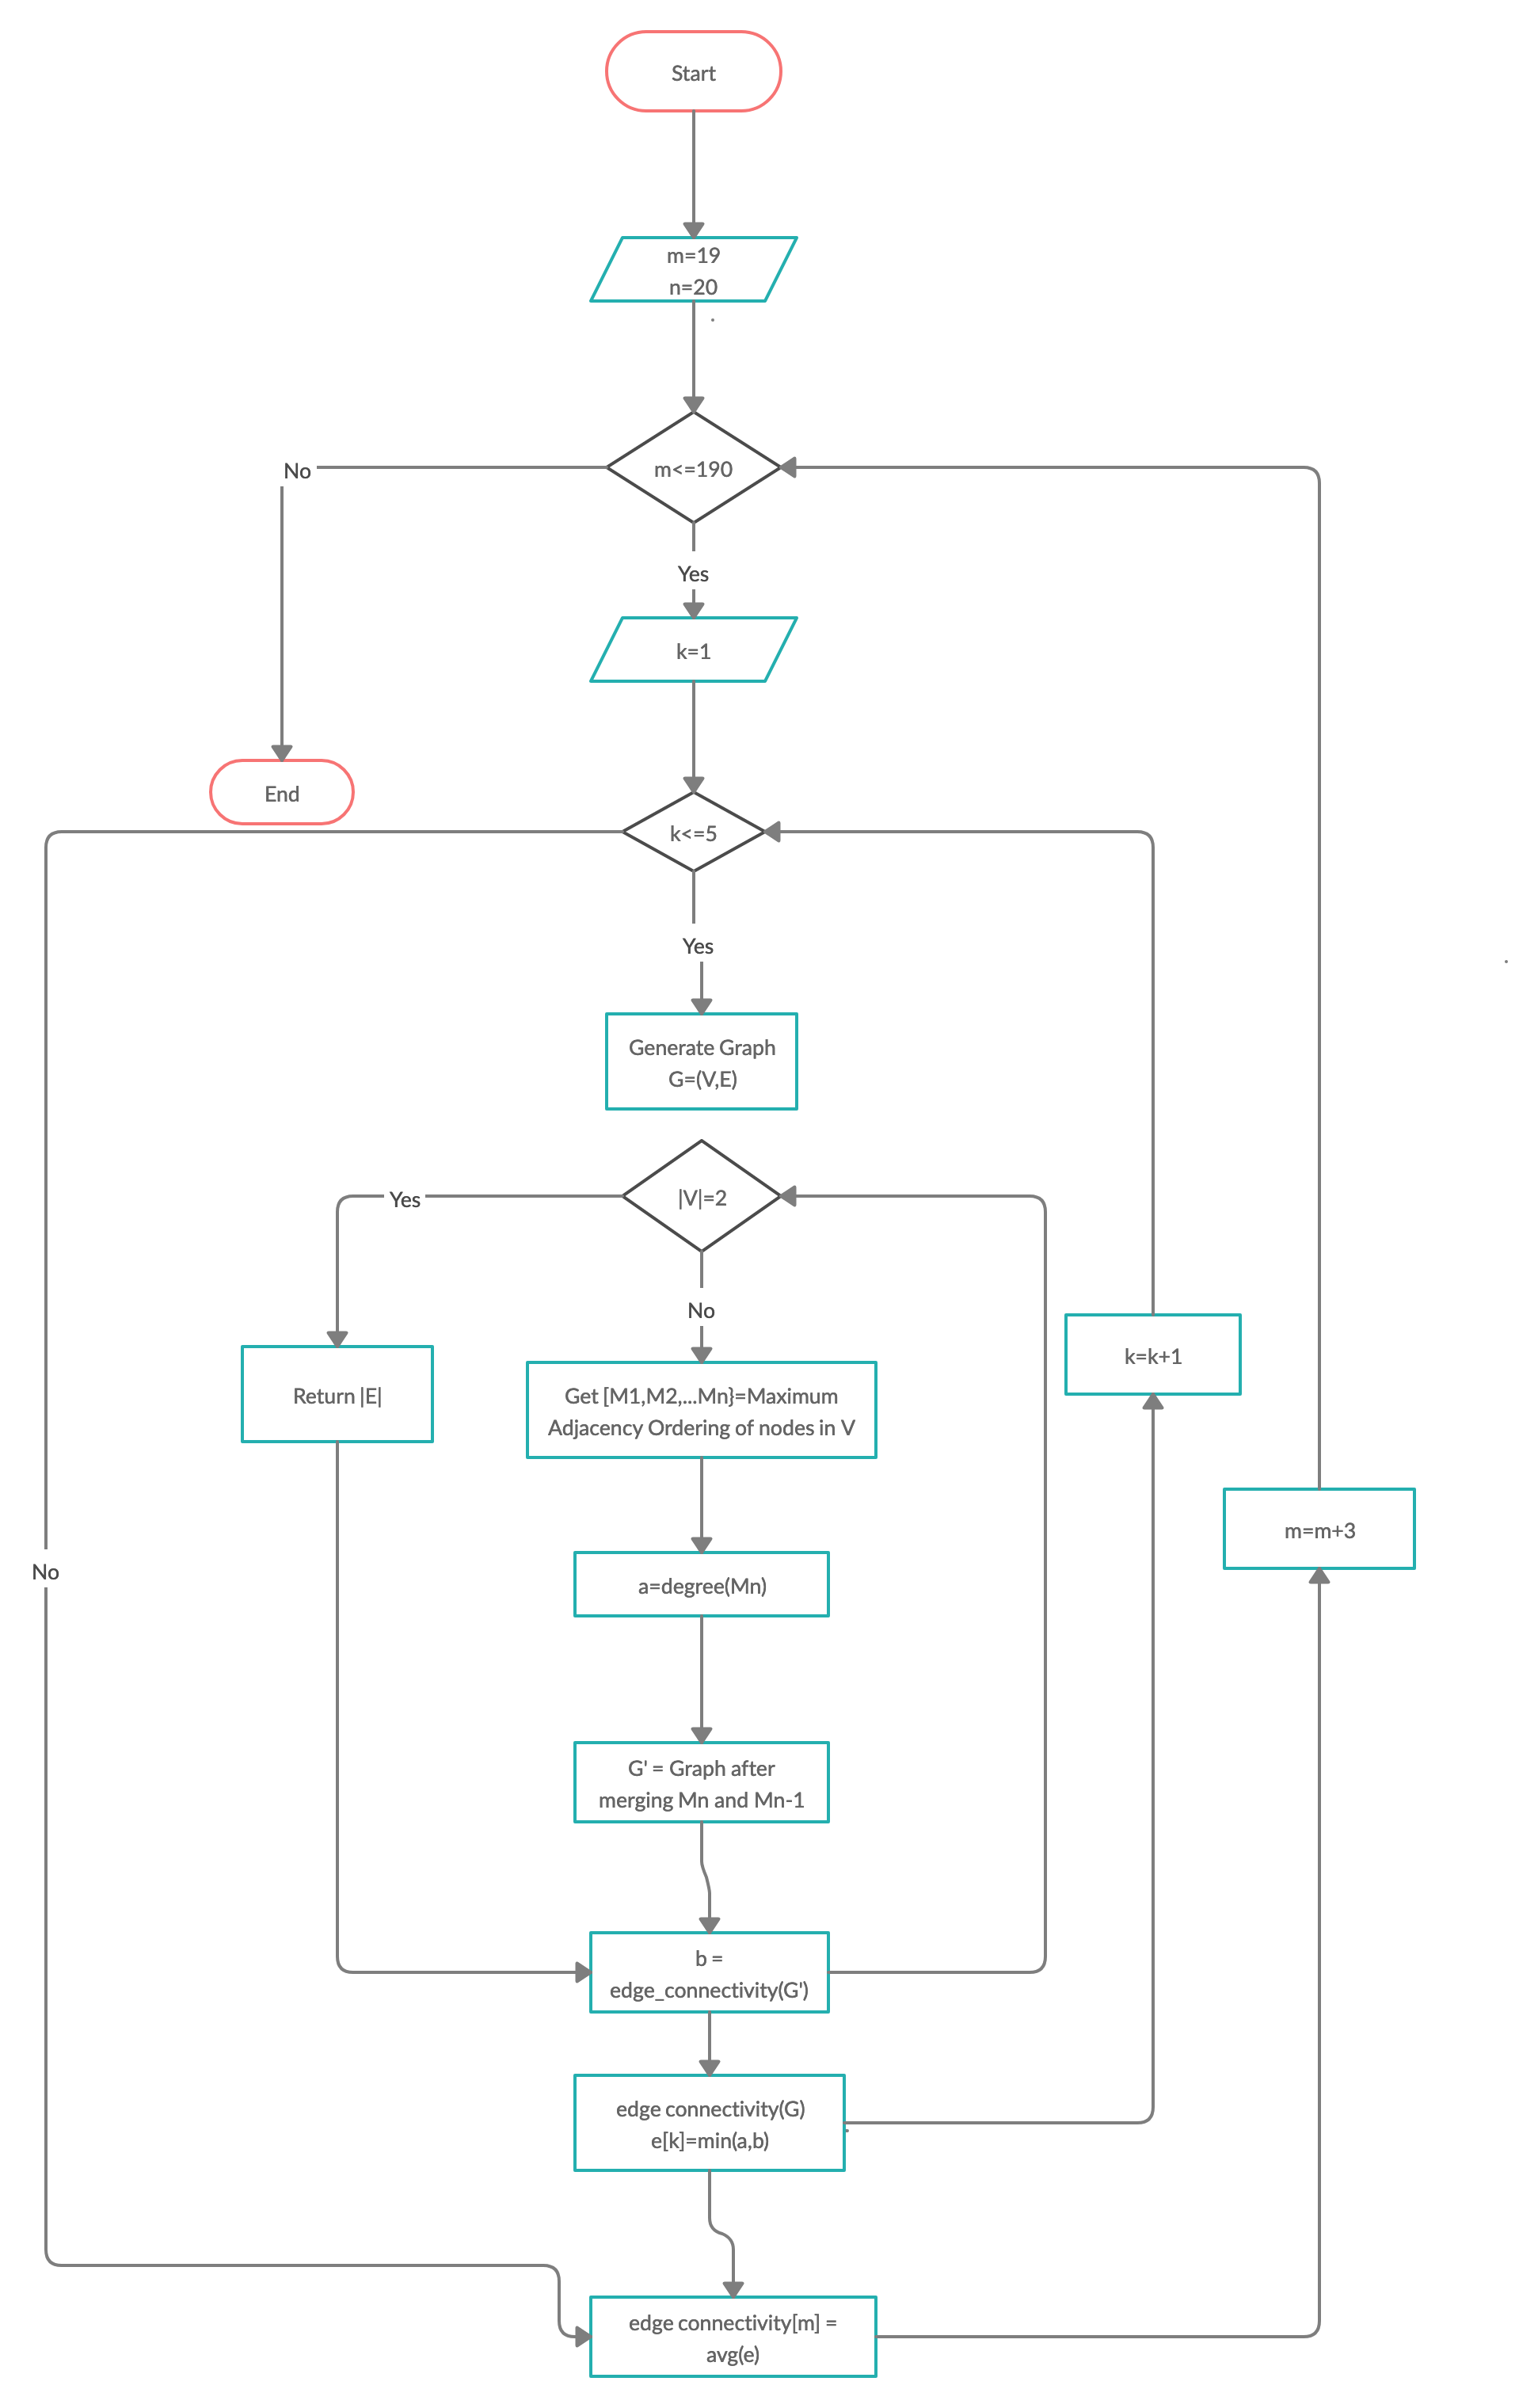
\includegraphics[scale=0.2]{fig/flowchart.png}
\end{itemize}


\section{Nagamochi Ibaraki Algorithm - Explanation}
\begin{itemize}


\item The goal is to find the \textit{edge connectivity} of a graph G=(V,E) i.e. the minimum number of edges which must be deleted to disconnect G

\item If the graph is not connected, its edge connectivity is \textbf{zero}
\item \textbf{Base Case}: There are only two nodes i and j in the graph, so the edge connectivity of the graph  is the number of edges (if any) between i and j

\item \textbf{Recursive Case}: 
\begin{itemize}
\item There are n nodes in the current graph, $n>=3$
\item We find the maximum adjacency ordering of the nodes in the current graph. Let it be $v_{1},v_{2},..v_{n-1},v_{n}$

\item We take the last two nodes in the above ordering, x=$v_{n-1}$ and y=$v_{n}$. Then, $a=\lambda(x,y$)= degree(y)

\item Merge nodes x and y into one node. Let $G_{xy}$ be the resulting graph.

\item Find the edge connectivity of $G_{xy}$. Let it be b.

\item Return min(a,b)



\end{itemize}








\begin{algorithm}[H]
    \caption{NagamochiIbarakiAlgorithm}
    \begin{algorithmic}[1]
        \Procedure{NagamochIbaraki}{$V,E$}
      
      \State $n= \mid V \mid$
      \If{$n=2$}
      \State return $\mid E \mid$
      \EndIf
      
        
        \State $[v_{1},v_{2},...v_{n}]$ = maximumAdjacencyOrdering(V)
        
        \State $x=v_{n-1}$
        \State $y=v_{n}$
        \State a=$degree(y)$
        \State$ G_{xy}$=graph created by merging nodes x and y
        \State b = NagamochiIbaraki$(V_{xy}, E_{xy})$
        \State return min(a,b)
        
     
     
      
        \EndProcedure
    \end{algorithmic}
    \end{algorithm}


\item The result  is the edge connectivity of the graph.

\end{itemize}

\section{Observations and Analysis}
\begin{itemize}


\item The program produces outputs as shown in the figures below.\\

 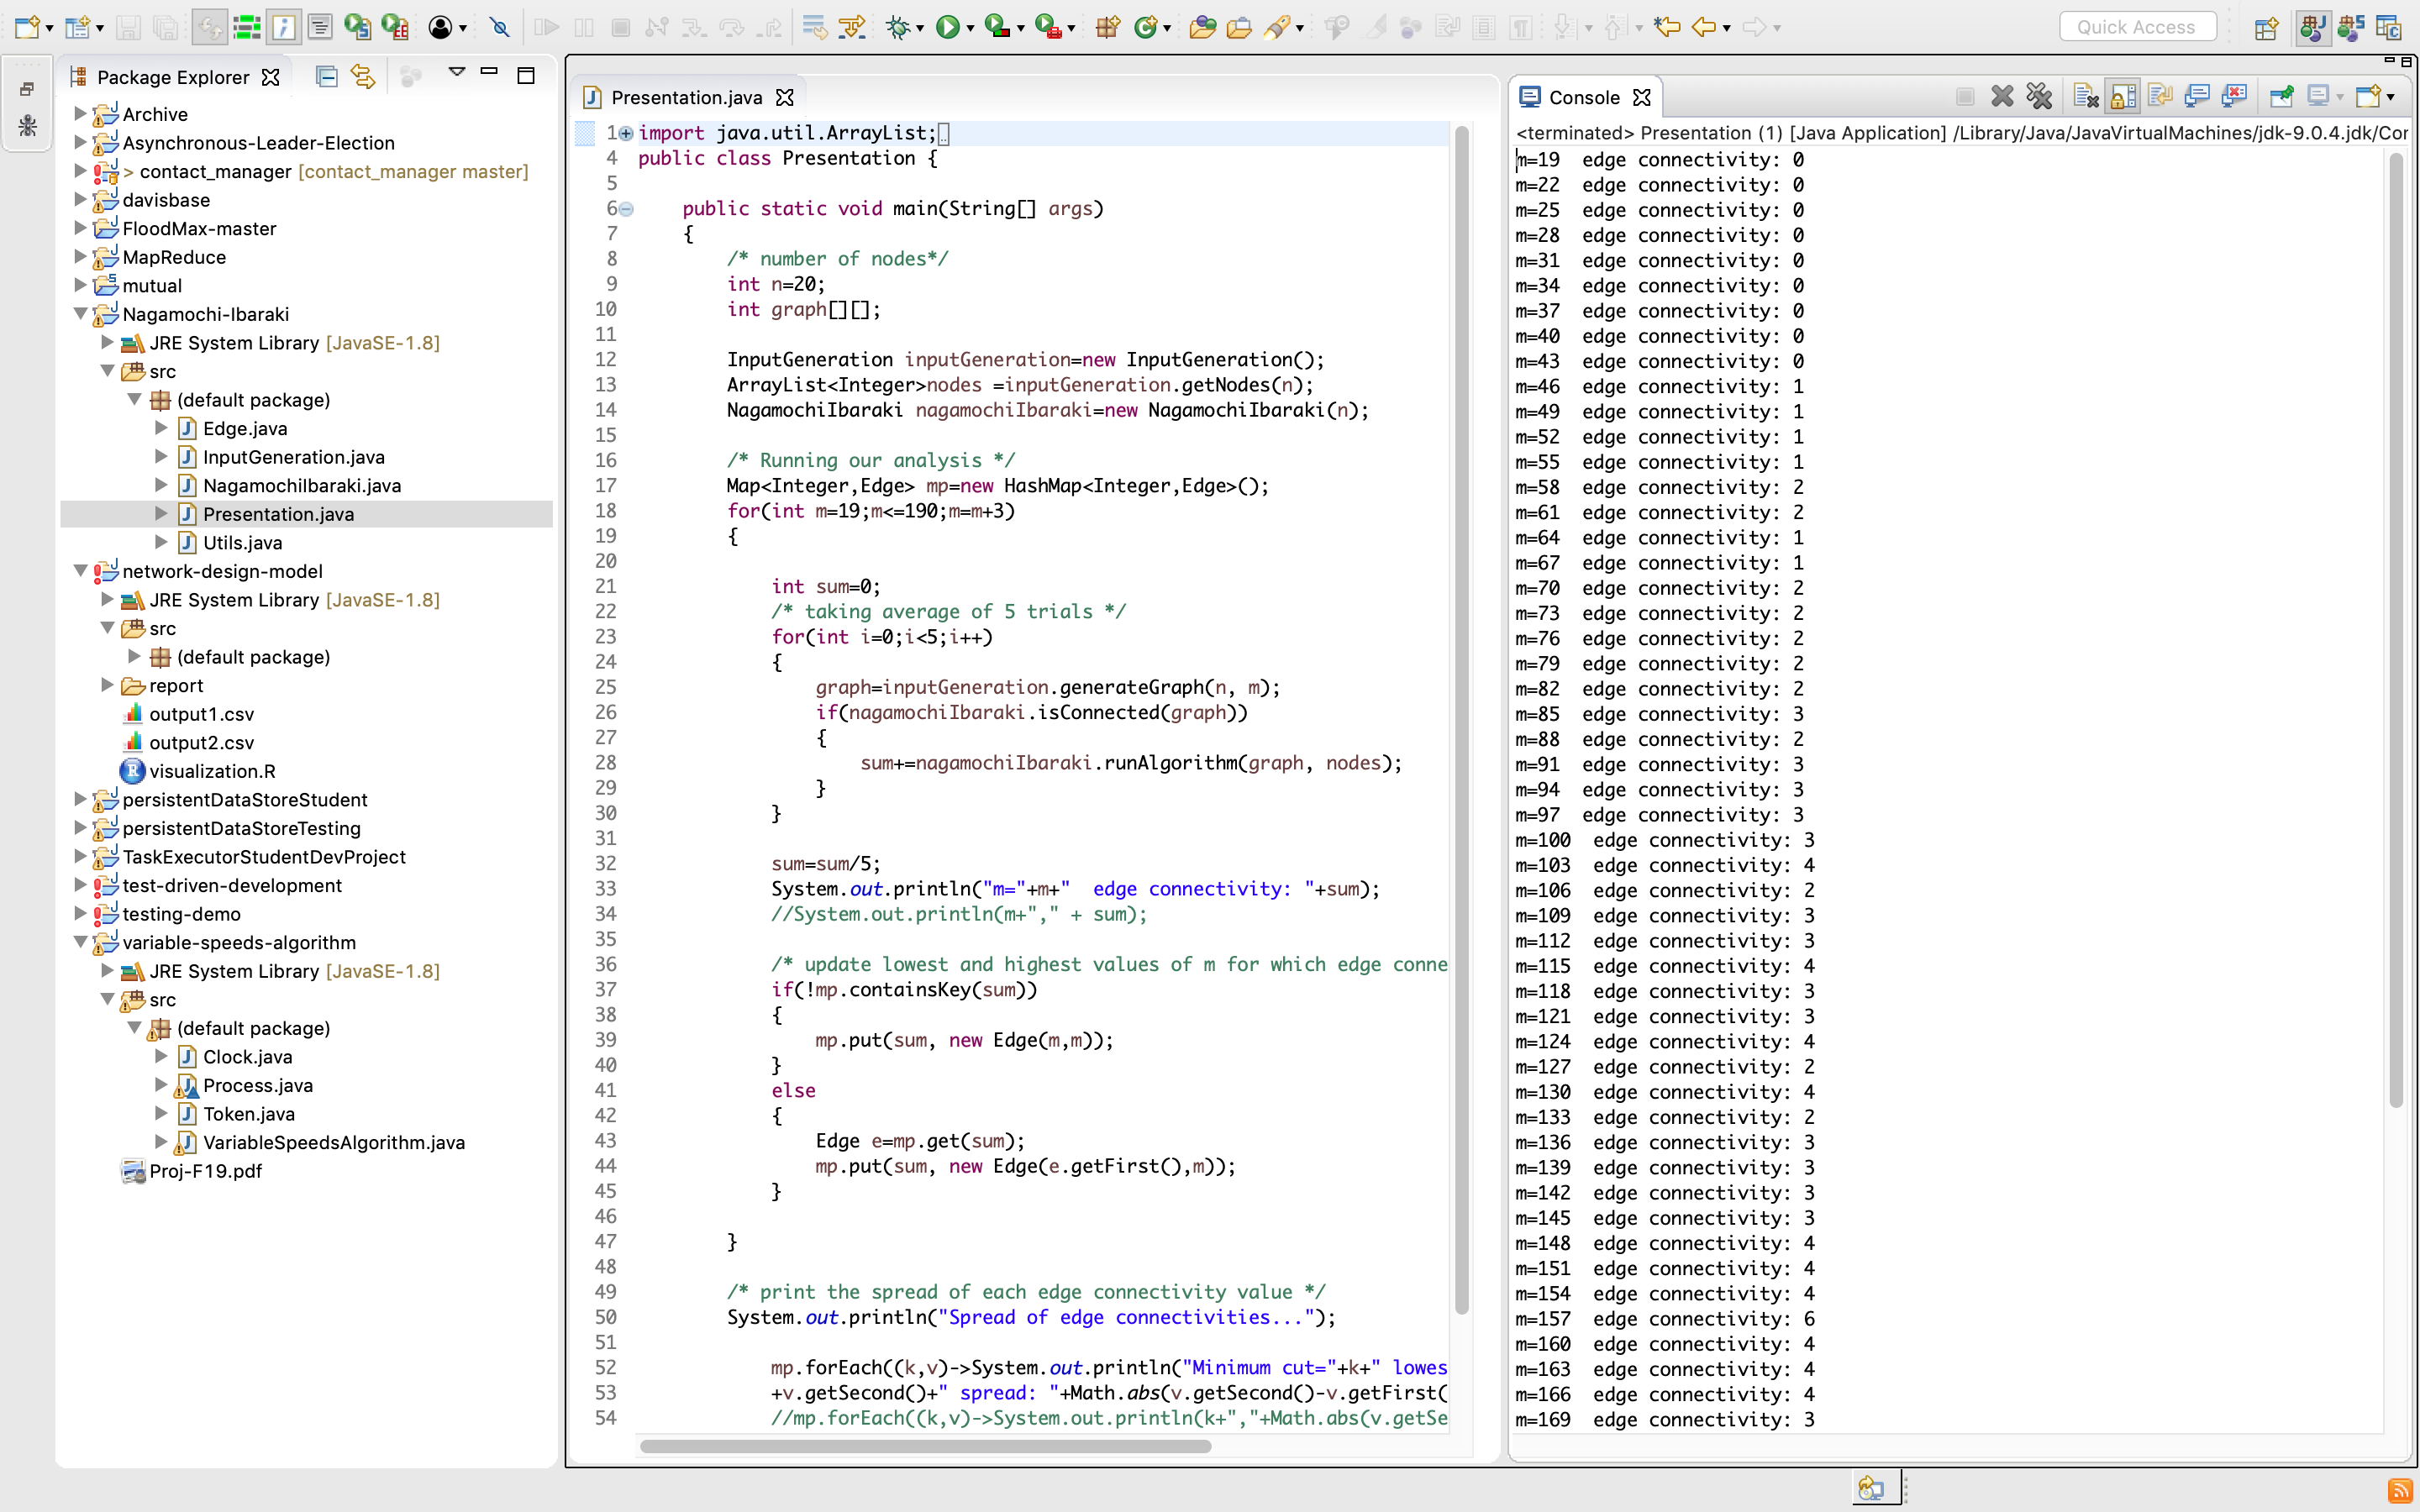
\includegraphics[scale=0.32]{fig/photo1.png}\\
 
  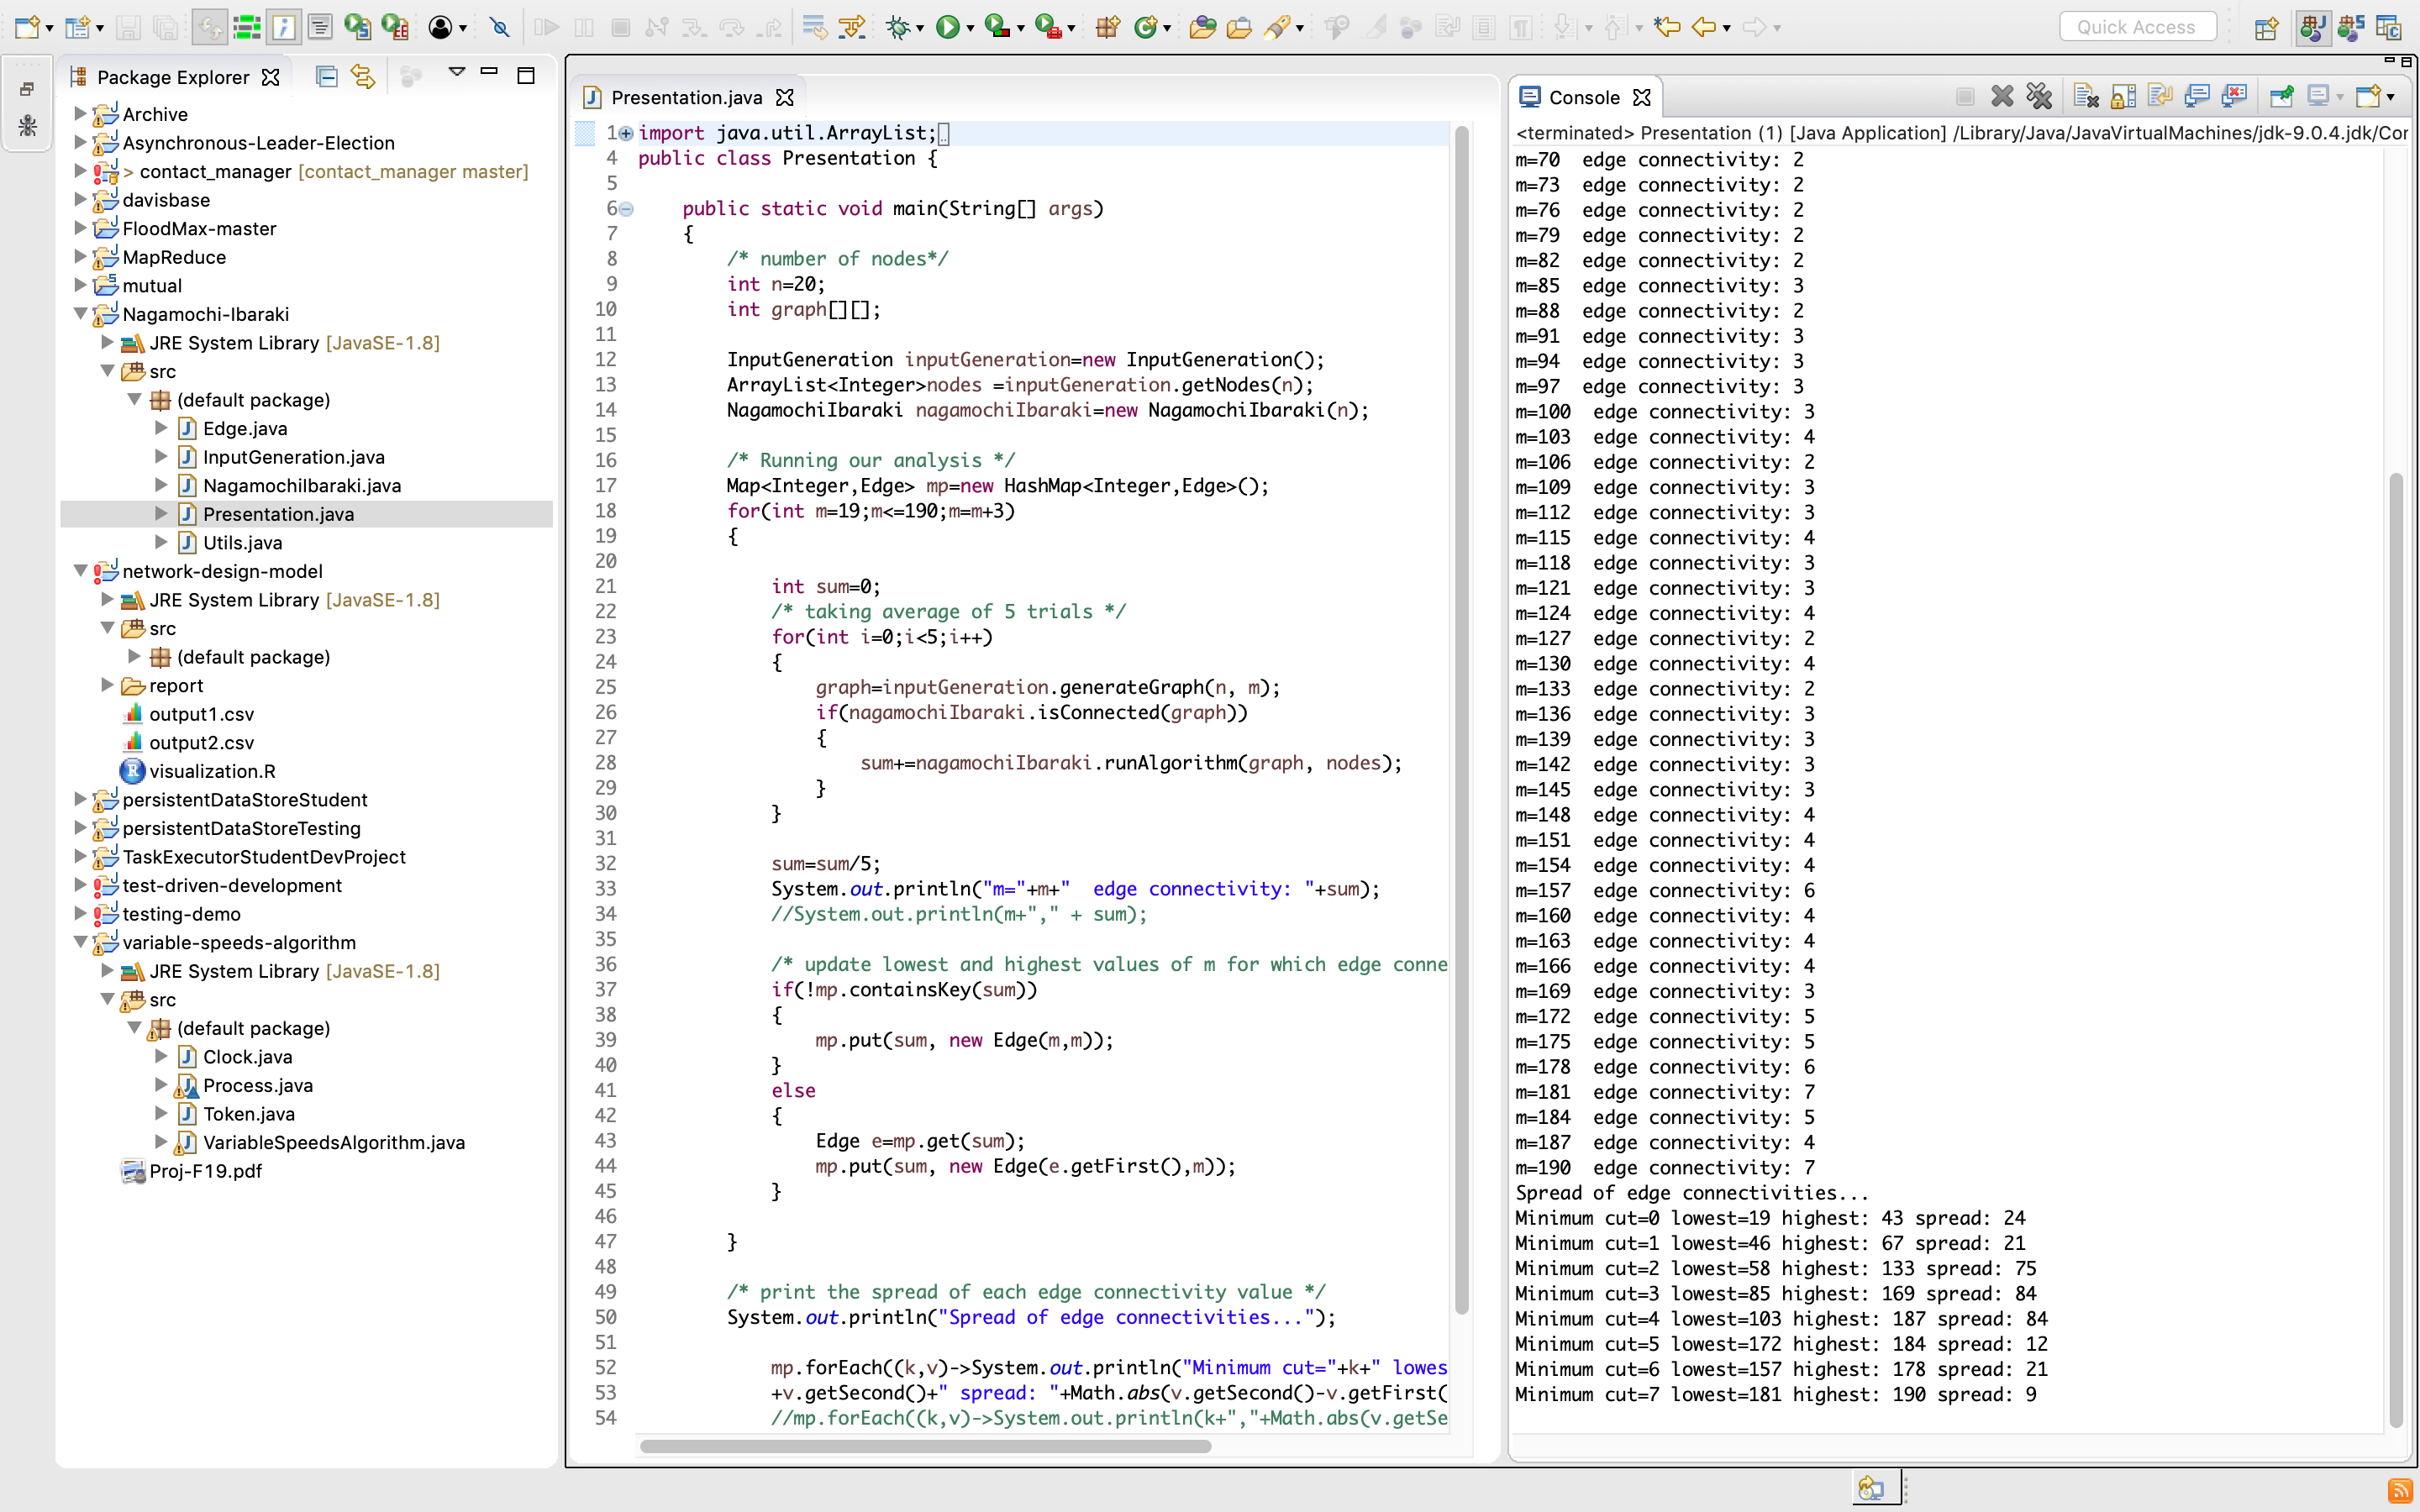
\includegraphics[scale=0.32]{fig/photo2.png}\\
 
\item The output results are stored in a \textit{csv} file. The graphs are generated in \textbf{R}.

\item We plot the graph of the \textit{number of edges} m vs. the \textit{edge connectivity} $\lambda(G)$

\includegraphics[scale=0.6]{fig/plot1.png}\\

\item We can clearly see that the edge connectivity of the network \textbf{increases} with increase in the value of m



\item We plot the graph of edge connectivity values \textbf{lambda(G)} against their \textbf{spread}\\

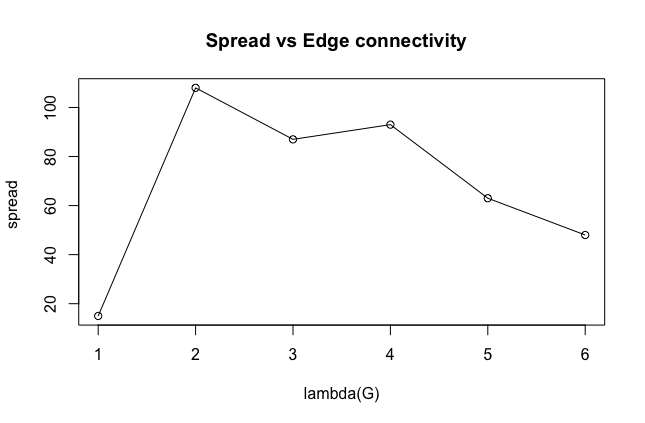
\includegraphics[scale=0.6]{fig/plot2.png}




\item We can clearly see that the \textbf{spread} of edge connectivity values increases, saturates in the middle and then decreases
\end{itemize}
 
\section{Discussion}
\begin{itemize}

\item As the number of edges in the graph increases, the number of edge disjoint paths between any two nodes tends to increase, hence the edge connectivity of the graph also \textbf{increases}

\item In our observations, the highest values of spread occur for $\lambda(G)=2,3,4$ with decreasing values on either side

\item The reason is that a given value of  edges connectivity (especially the ones in the middle) tends to persist for a range of m values, especially since for each graph we choose edges randomly, which sort of randomises our progression as m increases



\end{itemize}





  \section{ReadMe File}
  This section shows how to run the project files.
  \begin{itemize}
  \item Downloads the project files and store them in a folder
  \item Open the project folder in Eclipse
  \item Open the file \textbf{Presentation.java}
  \item Right Click $->$ Run as $->$ Java Application
  \item Alternatively,navigate to the folder in \textbf{terminal} and run the following commands
  \begin{itemize}
  \item javac Presentation.java
  \item java Presentation
  \end{itemize}
  \end{itemize}

  

 
\section{Code}

\textbf{Module 1: InputGeneration.java}
\lstinputlisting{/users/psprao/eclipse-workspace/Nagamochi-Ibaraki/src/InputGeneration.java}

\pagebreak
\textbf{Module 2: NagamochiIbaraki.java}
\lstinputlisting{/users/psprao/eclipse-workspace/Nagamochi-Ibaraki/src/NagamochiIbaraki.java}

\pagebreak
\textbf{Module 3: Presentation.java}
\lstinputlisting{/users/psprao/eclipse-workspace/Nagamochi-Ibaraki/src/Presentation.java}

\pagebreak
\textbf{Utils.java}
\lstinputlisting{/users/psprao/eclipse-workspace/Nagamochi-Ibaraki/src/Utils.java}

\textbf{Edge.java}
\lstinputlisting{/users/psprao/eclipse-workspace/Nagamochi-Ibaraki/src/Edge.java}

\textbf{Visualization.R.java}
\lstinputlisting{/users/psprao/eclipse-workspace/Nagamochi-Ibaraki/visualization.R}





\end{document}
